\section{Introduction}

Scalar active systems are those whose large scale nonequilibrium dynamics can be captured by a real (scalar) field, hereafter denoted $\phi$. 
The field $\phi$ is usually referred to as the \emph{order parameter} of the theory and can represent various quantities (see below). 
In many cases, though, it is related in various ways to the particle density.

At equilibrium, the minimal continuous description of scalar systems with conserved order parameter 
is achieved via \emph{model B} (see~\cite{HohenbergRMP} for a comprehensive classification).
Model B indeed describes a class of equilibrium systems whose dissipative dynamics is captured by a conserved field, such that $\intd{r} \, \phi(\bm r,t) = {\rm const} \; \forall t$, 
where hereafter the variables $\bm r$ and $t$ respectively account for space and time, while $d$ denotes the number of spatial dimensions.
As model B describes the universal large scale features of many systems, it can be formulated based on relevant symmetries and conservation laws.
Such phenomenological approach can moreover be supplemented by direct coarse-graining from microscopic (particle-based) theories which provide additional physical insights. 

In these notes, we will apply both approaches --phenomenological and coarse-grained-- to study the dynamics of scalar active systems. 
After reviewing the essentials of equilibrium phase separation physics as described by model B in Section~\ref{sec_PMB}, 
we will see how the latter can be generalized to active systems by relaxing constraints imposed for equilibrium dynamics such as free energy minimization or the fluctuation dissipation relation in Sections~\ref{sec_top_down} and~\ref{sec_BEC}.
In Section~\ref{sec_bottom_up}, we will then derive the coarse grained description of a minimal particle-based scalar active matter model,
which will allow us to uncover a physical origin for active phase separation, and show how it is markedly distinct from its counterpart at equilibrium.

\section{Passive model B and Cahn-Hilliard dynamics}

\label{sec_PMB}

\subsection{The dynamical theory for conserved scalar order parameter} 

We learnt from statistical mechanics that the large scale dynamics of systems which microscopically obey detailed balance minimizes a free energy.
Therefore, model B is generally written in terms of a functional ${\cal F}[\phi]$, whose expression can be generally\footnote{You can consider other terms up to order $|\nabla \phi|^2$, 
and then think of why they cannot be allowed in the expression of ${\cal F}$.} expressed as
\begin{equation} \label{eq_F}
{\cal F}[\phi] = \intd{r} \left[ f(\phi) + \frac{\kappa(\phi)}{2}|\nabla\phi|^2\right],
\end{equation} 
where we have kept terms up to order $|\nabla \phi|^2$.
In Eq.~\eqref{eq_F} $f$ denotes the `bulk' free energy density and $\kappa(\phi) > 0$ a generic constant.
The bulk contribution consists of a free energy landscape due to e.g.\ entropic effects and interactions between microscopic elements, 
while the $\kappa$ term describes the cost of interfaces.

The dynamical equation for $\phi$ then takes the general form
\begin{equation} \label{eq_phi}
\partial_t \phi(\bm r,t) = - \nabla \cdot \bm J(\phi) ,
\end{equation}
where the current $\bm J = \bm J_{\rm D} + \bm J_{\rm S}$ has a deterministic and stochastic contributions.
$\bm J_{\rm D}$ is set by the chemical potential:
\begin{equation} \label{eq_JD}
\bm J_{\rm D}(\phi) = - \bm M(\phi) \cdot \nabla \mu(\phi), \qquad \mu(\phi) = \frac{\delta {\cal F}}{\delta \phi} = f'(\phi) - \kappa(\phi) \nabla^2\phi - \frac{\kappa'(\phi)}{2}|\nabla\phi|^2 .
\end{equation}
The stochastic part $\bm J_{\rm S}$ can be determined using the fluctuation dissipation relation:
\begin{equation} \label{eq_JS}
\bm J_{\rm S}(\bm r,t) = \sqrt{2 k_B T} \bm \sigma(\phi) \cdot \bm \Lambda(\bm r,t), \qquad \Lambda_i(\bm r,t)\Lambda_j(\bm r',t') = \delta_{ij}\delta^d(\bm r - \bm r')\delta(t - t'),
\end{equation}
with $\sigma_{ik}(\phi)\sigma_{jk}(\phi) = M_{ij}(\phi)$ (Einstein summation is implied).

\noindent {\it Exercise: Show that Eqs.~(\ref{eq_phi}-\ref{eq_JS}) imply the stationary Boltzmann distribution ${\cal P}_{\rm s}[\phi] = \exp\left(-\tfrac{{\cal F}[\phi]}{k_B T} \right)$ for the stochastic field $\phi$. 
Hint: the Fokker-Planck equation associated with~\eqref{eq_phi} is given by 
\begin{equation*}
\partial_t {\cal P}[\phi,t] = \intd{x} \frac{\delta}{\delta \phi}\left[ \nabla \cdot \left( {\cal P}[\phi,t] \bm J_{\rm D} - k_B T \bm M(\phi) \cdot \nabla \frac{\delta}{\delta \phi} {\cal P}[\phi,t]  \right) \right] .
\end{equation*}
}

The stochastic contribution to Eq.~\eqref{eq_phi} is usually written to study dynamical effects due to fluctuations (such as the roughening of interfaces, or when one studies critical points using the dynamical renormalization group). In these lectures we will focus on the mean field properties of the models and thus drop the contribution from the noise ($\bm J_{\rm S} = \bm 0$).

In these notes, we will keep the expression of the free energy density $f(\phi)$ general. 
Its expression of course depends on the model of interest, below we describe two popular ones: 
\begin{itemize}
\item {\bf The Flory-Huggins theory of polymer solutions.} Considering polymers in a solvent with respective volume fractions $\phi = v \rho$ and $\phi_{\rm sol} = v_{\rm sol} \rho_{\rm sol}$, 
the incompressibility of the solution implies that $\phi + \phi_{\rm sol} = 1$.
The Flory-Huggins free energy is then given by
$f_{\rm FH}(\phi) = k_B T \left[ \tfrac{1}{v} \phi \ln(\phi) + \tfrac{1}{v_{\rm sol}} (1-\phi)\ln(1-\phi) \right] + \chi \phi(1-\phi)$ where the first term accounts for the entropy contribution due to mixing of the polymer in the solvent, while the second term ($\propto \chi$) accounts for interactions. In the case where the latter are attractive, $\chi < 0$. For more details see e.g.~\cite{Eisele1990}. 
\item {\bf Cahn-Hilliard (Landau).} In general, the free energy can expanded in powers of $\phi$: $f_{\rm CH}(\phi) = \sum_i \tfrac{a_k}{k}\phi^k$ with the $\{a_k\}$ real coefficients allowed by the symmetries of the problem. 
Such expansion is generally considered as formally valid close to a critical point where $\phi$ is small (typically $\phi = (\rho - \rho_c)/\rho_c$) such that one usually truncates it at order $k = 4$.
Note that $f_{\rm CH}$ can be obtained from $f_{\rm FH}$ by expanding the logarithms.
\end{itemize}

\subsection{Some elements on the physics of phase separation at equilibrium}

From now one and for simplicity, we will restrict the presentation to the case of a scalar mobility $M(\phi) > 0$.\\

\noindent {\it Spinodal decomposition} First, we can investigate the condition for a homogeneous configuration with $\phi = \bphi$ to be linearly stable.
Writing $\phi(\bm r,t) = \bphi + \delta \phi(\bm r,t)$, the perturbations $\delta \phi(\bm r,t)$ obey at linear order
\begin{equation} \label{eq_linear_phi}
\partial_t \delta \phi(\bm r,t) = \bar{M} \nabla^2 \left[ \left( \bar{f}'' - \bar{\kappa} \nabla^2\right)\delta \phi(\bm r,t)\right],
\end{equation}
where the bars stand for quantities evaluated at $\bphi$. 
Going into Fourier space, the growth rate associated to the mode with wavenumber $q$ is therefore $\lambda_q = -\bar{M} q^2(\bar{f}'' + \bar{\kappa} q^2)$.
As $\bar{M}$ and $\bar{\kappa}$ are both positive, the homogeneous configuration becomes unstable whenever $\bar{f}'' < 0$. 
This condition defines the so-called spinodals in the $(\bphi, k_B T$) phase diagram (Fig.~\ref{figeq}). \\

%%%%%%%%%%%%%%%%%%%%%%%%%%%%
\begin{figure}[t!]
	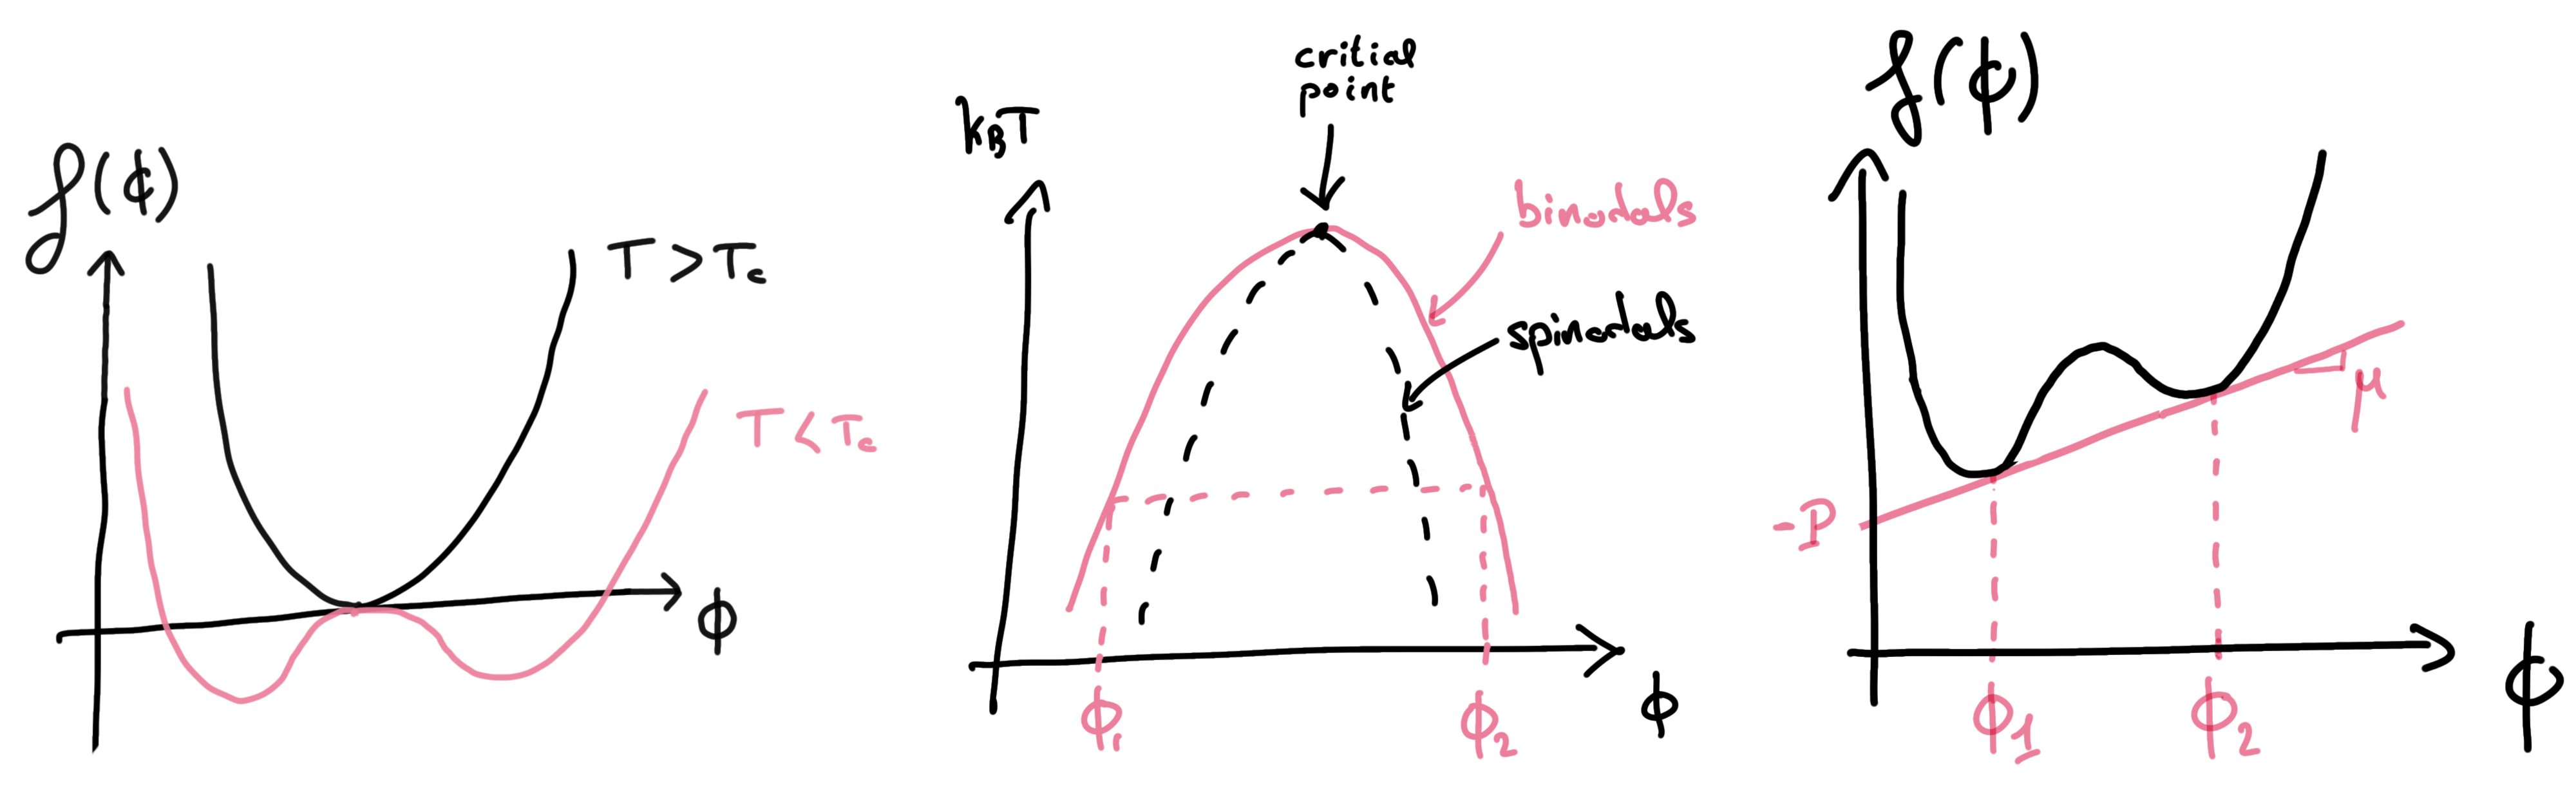
\includegraphics[width=\textwidth]{Figures/equilibrium_ps.pdf}
	\caption{Left: Typical Landau free energy landscapes above and below the critical point. 
	Center: phase diagram in the temperature $\phi$ plane showing the spinodals, binodals and critical point. 
	Right: Common tangent construction allowing to determine the coexistence densities in the phase separated regime.}
	\label{figeq}
\end{figure}
%%%%%%%%%%%%%%%%%%%%%%%%%%%%

\noindent {\it Binodals and the composition of phase separated configurations} 
The linear stability analysis and determination of the spinodals does not tell us anything about the asymptotic ($t \to \infty$) state of the system.
After the system undergoes spinodal decomposition, it goes through a coarsening regime until it phase separates into coexisting domains with different volumes and densities.
To determine the coexisting densities, we use the conservations of the total volume ${\cal V}$ and of the field $\phi$. 
We moreover work in the thermodynamic limit ${\cal V} \to \infty$ such that contributions from the interfaces can be safely neglected and we only consider the bulk contribution $f(\phi)$.
In a stationary phase separated regime where the system is partitioned into two domains with $\phi = \phi_{1,2}$ and of respective volumes ${\cal V}_{1,2}$, 
the free energy~\eqref{eq_F} thus takes the form
\begin{equation} \label{eq_F_ps}
{\cal F} = f(\phi_1) {\cal V}_1 + f(\phi_2) {\cal V}_2,
\end{equation} 
while denoting the mean value of $\phi$ as $\bphi$ the conservation constraints give
\begin{equation} \label{eq_constraints_binodals}
\phi_1 {\cal V}_1 + \phi_2 {\cal V}_2 = \bphi {\cal V}, \qquad  {\cal V}_1 + {\cal V}_2 = {\cal V} .
\end{equation} 
To determine the values $\phi_1$ and $\phi_2$, we can thus minimize the free energy~\eqref{eq_F_ps} imposing~\eqref{eq_constraints_binodals}.
This is done by adding the Lagrange multipliers ($\mu,P$) to ${\cal F}$, such that we define $\tilde{\cal F} = {\cal F} + P({\cal V}_1 + {\cal V}_2) - \mu(\phi_1 {\cal V}_1 + \phi_2 {\cal V}_2)$.
Minimizing $\tilde{\cal F}$ wrt the values of $\phi$ and volume for each of the two populations, we get
\begin{align} \label{eq_binodal_mu}
\frac{\partial \tilde{\cal F}}{\partial \phi_i}  & = {\cal V}_i (f'(\phi_i) - \mu) = 0 , \\
\label{eq_binodal_P}
\frac{\partial \tilde{\cal F}}{\partial {\cal V}_i}  & = f(\phi_i) - \mu \phi_i + P = 0 ,
\end{align}
with $i = 1,2$.
Eq.~\eqref{eq_binodal_mu} thus imposes that the chemical potential $\mu = f'(\phi_1) = f'(\phi_2)$ takes identical values in both phases (\emph{diffusive equilibrium}),
while Eq.~\eqref{eq_binodal_P} ensures the equality of pressures (\emph{mechanical equilibrium}).
Therefore, one can thus determine graphically the values of $\phi_1$ and $\phi_2$ from a common tangent construction 
on the free energy landscape. 
Indeed, the equality of chemical potentials imposes equal slopes of $f$ at $\phi_1$ and $\phi_2$, 
while equality of pressures imposes a common intercept on the vertical axis as shown in Fig.~\ref{figeq}

Varying e.g.\ the system temperatures, the coexistence values $\phi_{1,2}$ define the \emph{binodal curves},
and meet the spinodals we determined previously at the critical point. 
As shown in Fig.~\ref{figeq}, the spinodals and binodals generally do not coincide, such that there are regions of the phase diagram 
where phase separated configurations exist (and are stable) but the homogeneous state at $\phi = \bphi$ is also linearly stable.
In practice, if we now put back noise into the picture in these regions the homogeneous state will typically disappear 
not through the deterministic growth of an infinitesimal perturbation, 
but because of stochastic nucleation events which correspond to large perturbations and thus cannot be captured by linear stability analysis.
At fixed temperature below $T_c$ and for $\bphi$ lying in between the binodals, the system thus always phase separates over long times into two distinct domains 
where $\phi$ takes values $\phi_{1,2}$ and whose volumes linearly interpolate between 0 and ${\cal V}$ for $\bphi \in [\phi_1;\phi_2]$ due to the condition~\eqref{eq_constraints_binodals}, 
namely
\begin{equation}
{\cal V}_1 = \frac{\phi_2 - \bphi}{\phi_2 - \phi_1} {\cal V}, \qquad {\cal V}_2 = {\cal V} - {\cal V}_1 = \frac{\bphi - \phi_1}{\phi_2 - \phi_1} {\cal V},
\end{equation} 
which is known as the \emph{lever rule}.\\

\noindent {\it The coarsening dynamics} So far, we have discussed the linear instability of homogeneous solutions and the relative composition of phase separated phases.
Of course, another interesting aspect of phase separation concerns how one moves from one to the other. 
Without entering into details (for the interested reader see~\cite{Bray1994}), 
the coarsening process leading to phase separation can be understood by taking into account finite size effects, 
i.e.\ by considering the nonlocal contributions to the free energy which were neglected above.
Doing this, one finds that the pressure inside a spherical droplet increases with its interface curvature, 
leading to a diffusive flux from small to large droplets. 
Over long times, small droplets thus typically shrink at the expense of larger ones which is known as \emph{Ostwald ripening}.
One can moreover show that under this process the mean droplet radius universally grows as $\sim t^{1/3}$,
while the asymptotic ($t \to \infty$) state inevitably consists of two macroscopic phase separated domains. 

\section{Active model B: a top-down approach}

\label{sec_top_down}

In the previous section we have briefly reviewed the physics of phase separation at equilibirum using the minimal formulation offered by model B.
A general question now is how to generalize model B to the case where the microscopic dynamics of the system is active, 
i.e.\ breaks time-reversal symmetry at microscopic scales.
As we want to describe scalar active systems, we can reasonably conjecture (and we will show it later) that the dynamics of their density field should obey an equation similar to~\eqref{eq_phi}. 
Keeping a vanishing stochastic current, 
a straightforward way to break the equilibrium structure of Eq.~\eqref{eq_phi} consists in adding to the chemical potential in Eq.~\eqref{eq_JD} a contribution that cannot be derived from a free energy.
Considering reasonably smooth functions, we immediately see that any nonequilibrium contribution to $\mu$ must come from the nonlocal (proportional to the gradients of $\phi$) terms.
We can thus write in general
\begin{equation} \label{eq_neq_mu}
\mu(\phi) = f'(\phi) - \kappa(\phi) \nabla^2\phi + \lambda(\phi)|\nabla\phi|^2 ,
\end{equation}
such that when the relation $2\lambda(\phi) + \kappa'(\phi) \ne 0$ is not satisfied, $\mu$ cannot be written as $\delta {\cal F}/ \delta \phi$.
While only the local term $f'(\phi)$ in~\eqref{eq_neq_mu} affects the evaluation of the spinodals, 
the absence of free energy structure prevents us to use the powerful formalism presented above to determine the binodals and thus the phase separated configurations.

Fortunately, as was demonstrated in~\cite{Solon2018} an effective free energy structure can be recovered through a mapping of $\phi$ and ${\cal F}$ to generalized thermodynamic variables.
Namely, let us consider the one to one mapping $\phi\to\psi$ and the functional ${\cal G}$ such that $\mu = \delta{\cal G}/\delta\psi$.
Writing, ${\cal G} = \intd{r} [g(\phi) + \tfrac{1}{2}B(\phi)|\nabla\psi|^2]$, we get
\begin{equation}
\frac{\delta {\cal G}}{\delta \psi} = \frac{g'(\phi)}{\psi'(\phi)} +\frac{1}{2}\frac{B'(\phi)}{\psi'(\phi)}|\nabla\psi|^2 - \nabla \cdot ( B(\phi)\nabla\psi) ,
\end{equation}
where primes denote derivatives wrt $\phi$.
Using that $\nabla\psi = \psi'\nabla\phi$, we obtain after straightforward algebra
\begin{align}
\mu & = \frac{g'(\phi)}{\psi'(\phi)} - B(\phi) \psi'(\phi) \nabla^2\phi  - \left[\psi''(\phi) B(\phi) + \frac{1}{2} B'(\phi)\psi'(\phi)\right]|\nabla\phi|^2 \\
& = f'(\phi) - \kappa(\phi) \nabla^2\phi + \lambda(\phi) |\nabla\phi|^2. \nonumber
\end{align}
Equating the rhs of the above expressions term by term, we thus get
\begin{equation}
g(\phi) = \int^\phi \rmd\tilde{\phi} \, f'(\tilde{\phi}) \psi'(\tilde{\phi}) , \qquad
B(\phi) = \frac{\kappa(\phi)}{\psi'(\phi)} , \qquad
\kappa(\phi)\psi''(\phi) = -[2\lambda(\phi) + \kappa'(\phi)]\psi'(\phi).
\end{equation}
You can check that that in the case $2\lambda(\phi) + \kappa'(\phi) = 0$ the third equality above implies without much surprise that $\psi = \phi$ up to a constant term which can be set to zero without loss of generality.
From the above, the dynamics of $\phi$ can now be written as minimizing a free-energy-like functional:
\begin{equation}
\partial_t \phi = \nabla\cdot \left[ M (\phi) \nabla\frac{\delta {\cal G}}{\delta\psi}\right] ,
\end{equation}
but where, in contrast with the equilibrium case, the minimization of ${\cal G}$ is performed over the auxiliary variable $\psi$ and not $\phi$ itself. 

\noindent {\it Exercise: Derive the equation governing the dynamics of $\psi$, what is the essential difference between it and the equilibrium model B?}\\

To identify the generalized pressure, we now note that the dynamics of $\phi$ can be generally expressed in terms of the stress tensor $\bm T$:
\begin{align}
\partial_t \phi & = \nabla\cdot \left [M(\phi) \nabla \frac{\delta {\cal F}}{\delta\phi} \right] = -\nabla\cdot\left[ \frac{M(\phi)}{\phi} \nabla \cdot \bm T\right] , \nonumber \\
\label{eq_stress}
T_{ij} & = \delta_{ij} \left[ F - \phi\frac{\delta {\cal F}}{\delta\phi} \right] - \frac{\partial F}{\partial (\partial_j \phi)}\partial_i \phi ,
\end{align}
with $F(\phi,\nabla\phi)$ defined from ${\cal F} = \intd{r} F$.

\noindent{\it Exercise: Demonstrate Eq.~\eqref{eq_stress}.}\\

It appears clearly from Eq.~\eqref{eq_stress} that the local diagonal part of the stress tensor corresponds to the pressure as defined from Eq.~\eqref{eq_binodal_P},
while in general the nondiagonal part defines an anisotropic pressure.
Therefore, neglecting nonlocal contributions as in the previous section we conclude from the above mapping that the generalized pressure for the active model B reads
\begin{equation} \label{eq_genP}
\Pi = \psi \mu  - g(\psi) =  \psi \frac{\rmd g}{\rmd \psi} - g(\psi) .
\end{equation}
Together, equalities of pressure and chemical potential between both phases therefore define a common tangent construction in terms of the variables $\psi$ and $g$ which
allows to determine the binodal densities and consequently the volume of each phase. 
The resulting phase diagram for active model B is therefore similar to the equilibirum one shown in Fig.~\ref{figeq}.

Similarly to equilibrium, taking into account finite size effects one can show that in this case the generalized pressure~\eqref{eq_genP} follows the Laplace law, 
such that the coarsening in active model B defined from Eq.~\eqref{eq_neq_mu} is also driven by Ostwald ripening.

Overall, the phenomenology of active model B (AMB) is similar to that of phase separation at equilibrium as it also admits a generalized free-energy-like structure. 
However, the generalized thermodynamic variables defined in this section do not carry any obvious mechanical interpretation and should only be seen as 
a convenient calculation framework to study the active phase separation physics.
These similarities to equilibrium are thus mostly due to the fact that time-reversal symmetry is broken in AMB in a `minimal way',
while of course other nonequilibrium contributions can be added to the current~\eqref{eq_JD} which might have much more dramatic effect.

An example worth mentioning here is the active model B+~\cite{Tjhung2018PRX} for which the current~\eqref{eq_JD} includes a term
\begin{equation}\label{eq_AMB_plus}
\bm J^{\rm AMB+}_{\rm D} = \zeta(\phi) (\nabla^2\phi) \nabla\phi ,
\end{equation}
that cannot be written as deriving from a generalized chemical potential.
This new term changes qualitatively the structure of the problem as it 
allows for non-curl-free currents ($\nabla \times \bm J \ne \bm 0$) in the steady state.
Such feature leads to qualitative changes in the phenomenology of active phase separation,
in particular the study of curved interfaces shows that $\bm J^{\rm AMB+}_{\rm D}$ is responsible for the emergence of negative interfacial tension, 
leading to reversed Ostwald ripening selecting a preferred (finite) droplet radius.

\section{Bose-Einstein-like physics in scalar active matter}

\label{sec_BEC}

\subsection{The diffusivity edge class}

In this section we discuss another class of nonequilibrium systems whose active nature lies in the explicit breaking of the fluctuation dissipation theorem (FDT).
Indeed, let us consider a diffusive dynamics in the presence of an externally applied potential $U$. 
At equilibrium, the corresponding (deterministic) current simply reads\footnote{Assuming FDT, what are the free energy functional and chemical potential corresponding to Eq.~\eqref{eq_currentU}?}
\begin{equation} \label{eq_currentU}
\bm J(\phi) = -M(\phi) \phi \nabla U - D(\phi) \nabla\phi ,
\end{equation}
where FDT implies that the effective diffusion coefficient is related to the mobility via the surrounding medium temperature: $D(\phi) = M(\phi) k_B T$.
In presence of activity, this relation does in general not hold and one is in principle allowed to consider arbitrary values for the ratio $D(\phi) / M(\phi)$.

Namely, we now consider a scalar density field whose dynamics is described by the current~\eqref{eq_currentU} while
the diffusivity over mobility ratio takes the general form
\begin{equation}
\frac{D(\phi)}{M(\phi)} = k_B \Teff \vartheta(\phi),
\end{equation}
where the subscript `eff' highlights that $\Teff$ does not correspond to a temperature in the thermodynamic sense, 
but should rather be interpreted as a control parameter for the dynamics.
Due to the absence of FDT, the function $\vartheta(\phi)$ is general but nonetheless assumed positive ($\vartheta(\phi) \ge 0$), 
while $\vartheta(\phi = 0) = 1$ such that $k_B \Teff$ can be viewed as an effective temperature for the system in the dilute limit.

On a physical viewpoint, the $\phi$ dependency of $\vartheta$ usually results from the integration of pairwise interactions between the particles.
Increasing (resp.\ decreasing) $\vartheta$ can thus be interpreted as collective inhibition (resp.\ activation) caused by the interplay of activity and interactions.
Moreover, as both $M$ and $\vartheta$ in general remain positive nonlocal contributions giving rise to higher order gradient terms in Eq.~\eqref{eq_currentU} are neglected.
As we discuss below, an interesting subclass of systems are those which exhibit a \emph{diffusivity edge}, 
i.e.\ those for which $\vartheta(\phi)$ is identically zero for $\phi$ above a certain threshold value $\phi_c$~\cite{GolestanianBEC}.

\subsection{The steady state solution}

In absence of external currents, the steady state configuration is obtained by setting $\bm J = \bm 0$,
which for $M(\phi) > 0$ implies the following relation between the density and the potential $U$:
\begin{equation} \label{eq_sol_diff_edge}
\frac{{\rm d}\beta U}{{\rm d}\phi} = -\frac{\vartheta(\phi)}{\phi},
\end{equation}
where we have defined $\beta \equiv (k_B\Teff)^{-1}$.
As $\vartheta(\phi) \ge 0$, we see from~\eqref{eq_sol_diff_edge} that $\phi$ is always a decreasing function of $U$. 
We thus denote $\phi_0$ as the maximal value that $\phi$ takes in the ground state $U=0$.
Integrating Eq.~\eqref{eq_sol_diff_edge} consequently leads to the following expression for the potential
\begin{equation} \label{eq_sol_diff_edge_2}
\beta U(\phi) = -\int_{\phi_0}^{\phi} {\rm d}\varphi \, \frac{\vartheta(\varphi)}{\varphi} .
\end{equation}
When $\phi_0 < \phi_c$, $\phi(U)$ can be obtained simply by performing the integral and inverting Eq.~\eqref{eq_sol_diff_edge_2}.

\noindent{\it Exercise: for $\vartheta(\phi) = 1$ which familiar distribution is recovered? Give a simple interpretation of this result.}\\

The integration constant $\phi_0$ is then determined from the density normalization, namely
\begin{equation} \label{eq_diff_edge_defN}
N = \intd{r} \phi(U(\bm r)) .
\end{equation}
with $N$ the total number of particles.
We now consider the case where the potential is harmonic: $U(\bm r) = \tfrac{k}{2}r^2$, such that we can rewrite the normalization condition~\eqref{eq_diff_edge_defN} as
\begin{equation} \label{eq_diff_edge_N}
N = {\cal S}_d \int_0^{\infty} \rmd r \, r^{d-1}\phi(U(r)) = \int_0^{\infty} \rmd U \, g(U) \phi(U).
\end{equation}
where ${\cal S}_d = 2 \pi^{d/2}/\Gamma(d/2)$ denotes the surface of the unit sphere embedded in $d$ dimensions,
while the second equality was obtained via the change of variable $r \to U$ and the density of state is given by 
\begin{equation} \label{eq_density_state}
g(U) = {\cal S}_d r^{d-1}(U)\tfrac{\rmd r}{\rmd U} = \frac{(2\pi)^{d/2}}{\Gamma\left(d/2\right)}\frac{U^{d/2-1}}{k^{d/2}}.
\end{equation}

We now use the fact that the density $\phi$ varies monotonously with $U$ to apply the change of variable $U \to \phi$
such that Eq.~\eqref{eq_diff_edge_N} is recast as
\begin{equation} \label{eq_diff_edge_N2}
N = \frac{k_B \Teff}{\Gamma(d/2)}\left(\frac{2\pi}{k}\right)^{\tfrac{d}{2}} \int_0^{\phi_0} \rmd \varphi \, U^{d/2-1}(\varphi) \vartheta(\varphi) \quad (\phi_0 < \phi_c).
\end{equation}
The expression given in Eq.~\eqref{eq_diff_edge_N2} is of course only valid for $\phi_0 < \phi_c$, i.e.\ when all the density profile takes values below the diffusivity edge. 
In the opposite case of $\phi_0 \ge \phi_c$, 
the integrand in Eq.~\eqref{eq_diff_edge_N2} vanishes identically in the interval $[\phi_c,\phi_0]$ and no longer contributes, 
which makes it impossible for the normalization to be satisfied. 
This feature can be traced back from Eq.~\eqref{eq_sol_diff_edge} to the fact that the profile $\phi(U)$ develops a vertical tangent at $U = 0$ for $\phi_0 \ge \phi_c$ (see Fig.~\ref{fig_BEC}(a)),
which can be interpreted as the creation of a singular condensate at the ground state of the potential.

It is easily shown from Eq.~\eqref{eq_diff_edge_N2} that $\phi_0$ is a decreasing function of 
$\Teff$ $({\rm d}\phi_0/{\rm d}\Teff \le 0)$.
Therefore, the normalization~\eqref{eq_diff_edge_N2} only holds for $\Teff  > T_c$, 
where $T_c$ is defined as the value of $\Teff$ for which $\phi_0$ reaches $\phi_c$.
In the condensation regime, the normalization of the stationary distribution requires to consider the contribution of the condensate separately.
Namely, denoting $N_c$ as the total number of particles in the condensate Eq.~\eqref{eq_diff_edge_N2} becomes for $\Teff \le T_c$, 
\begin{equation} \label{eq_diff_edge_Ncond}
N = N_c + \frac{k_B \Teff}{\Gamma(d/2)}\left(\frac{2\pi}{k}\right)^{\tfrac{d}{2}} \int_0^{\phi_c} \rmd \varphi \, U^{d/2-1}(\varphi) \vartheta(\varphi) \quad (\phi_0 \ge \phi_c).
\end{equation}
To simplify this expression, we note that for for $\Teff \le T_c$ Eq.~\eqref{eq_sol_diff_edge_2} implies that $\beta U$ is a function of $\phi/\phi_c$.
Denoting $u(\phi/\phi_c) = \beta U(\phi)$ as well as $\vartheta(\phi) \to \vartheta(\phi/\phi_c)$, and noting that $N_c = 0$ for $\Teff = T_c$,
Eq.~\eqref{eq_diff_edge_Ncond} is simplified as
\begin{equation} \label{eq_diff_edge_Ncond2}
\frac{N_c}{N} = 1 - \left( \frac{\Teff}{T_c}\right)^{\tfrac{d}{2}} \qquad (\Teff \le T_c),
\end{equation}
with 
\begin{equation*}
k_B T_c =  \frac{k}{2\pi} \left( \frac{\phi_c \int_0^1{\rm d}s\; \vartheta\left( s \right) u^{d/2 - 1}(s) }{N \, \Gamma(d/2)} \right)^{-\tfrac{2}{d}} .
\end{equation*}

Note that, in contrast with passive and active phase separation, the condensation phenomenon described here requires the system to evolve in a potential landscape.
Indeed, setting $U(\bm r)=0$ in Eq.~\eqref{eq_currentU} one can check that the diffusivity edge is unable to trigger an instability of homogeneous configurations, even for $\bphi > \phi_c$.

%-----------------------------------------------------------------------------------------------------------%
\begin{figure}[t!]
	\centering
	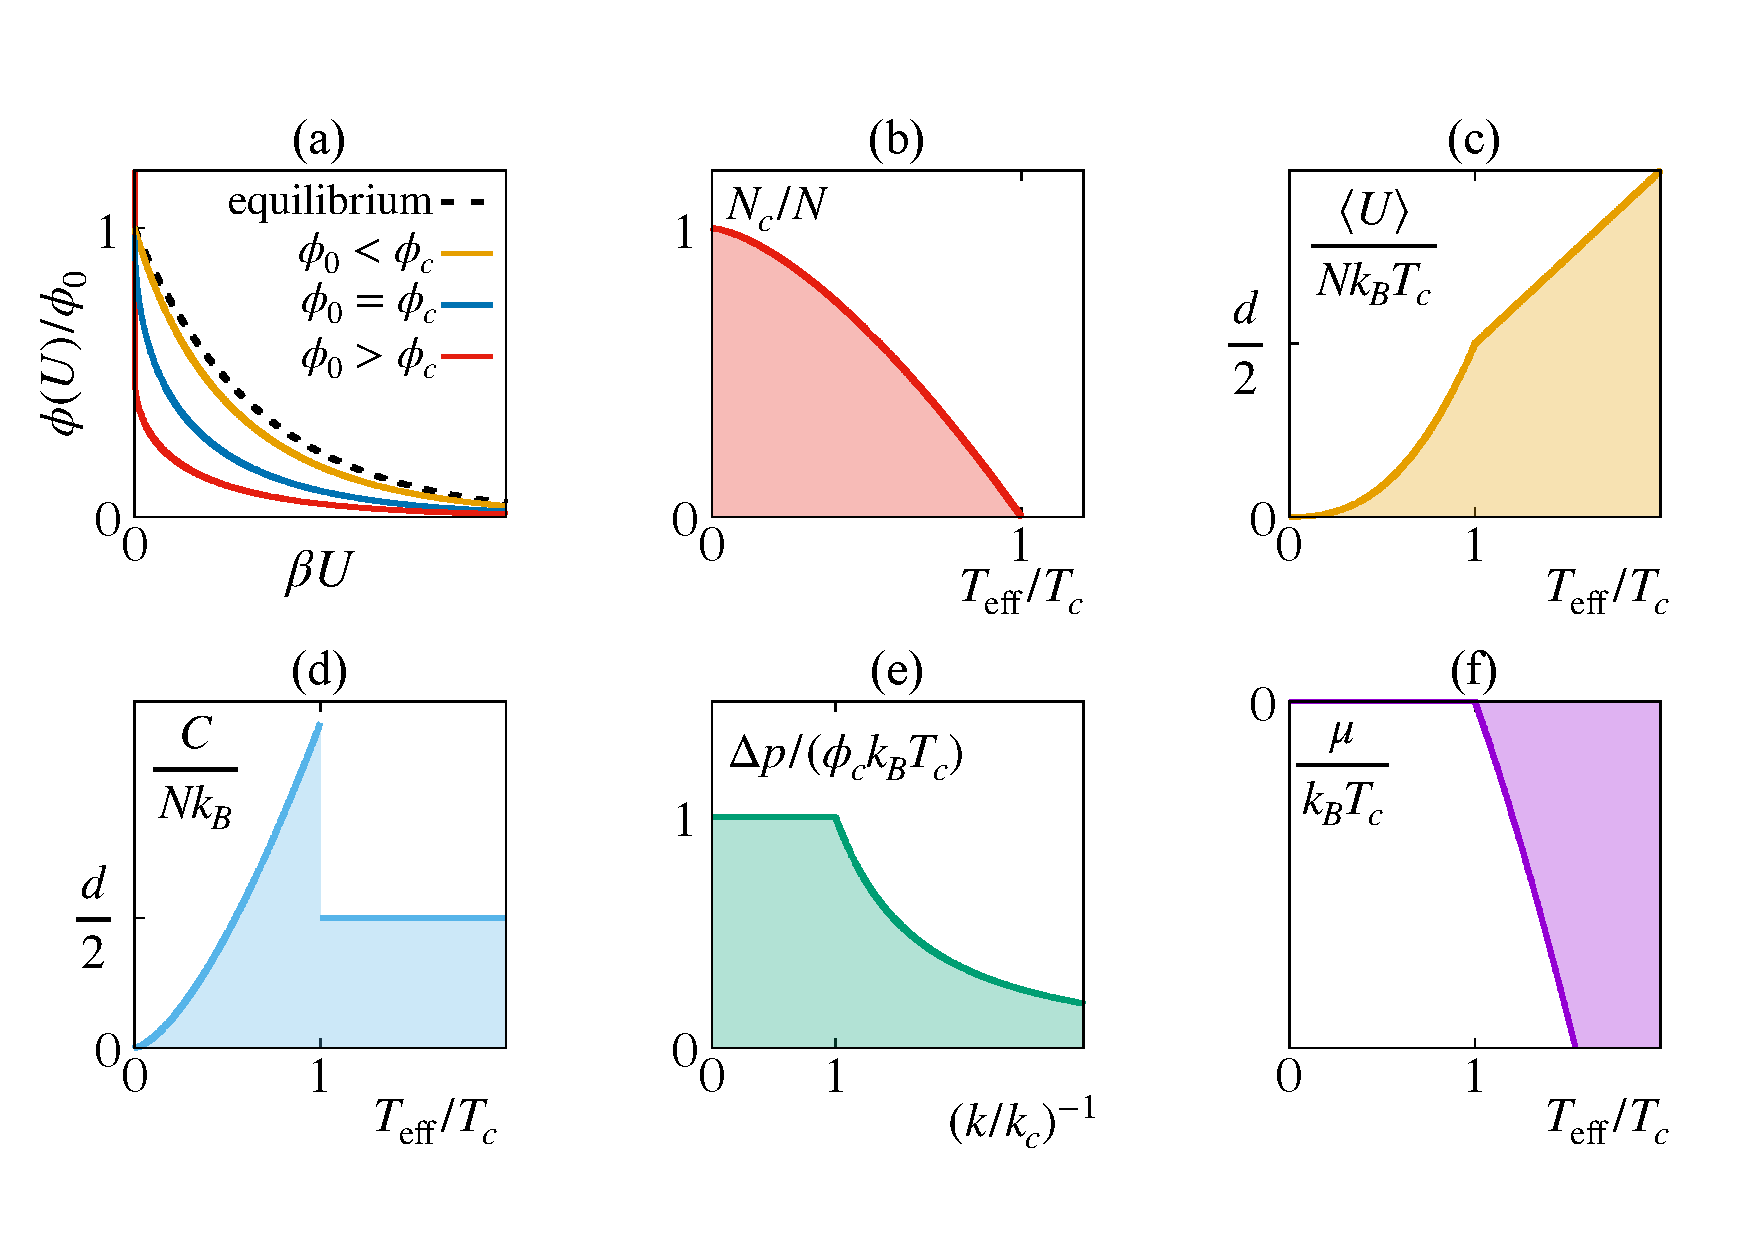
\includegraphics[width = .75\textwidth]{Figures/Fig_BEC.pdf}
	\caption{The diffusivity edge induced condensation.
	(a) The steady state density for different values of $\phi_0/\phi_c$.
	(b) The fraction of particles in the condensate as function of the effective temperature.
	(c-f) The thermodynamics of condensation for a step function diffusivity profile:
	average energy (c), heat capacity (d) and chemical potential (f) as function of $\Teff/T_c$,
	(e) pressure isotherm computed by varying the potential stiffness $k$.}
	\label{fig_BEC}
\end{figure}
%-----------------------------------------------------------------------------------------------------------%

\subsection{The thermodynamics of condensation}

Remarkably, although the diffusivity edge condensation has a purely nonequilibrium origin, as for AMB it still admits an effective thermodynamic description.
In this section, we will detail the properties of the condensation transition outlined above by deriving the appropriate thermodynamic framework.



While this can be done for the general case, 
for the sake of clarity we will focus here on the case where the function $\vartheta(\phi/\phi_c)$ is equal to one for $\phi/\phi_c < 1$ and zero otherwise.
Formally, 
\begin{equation} \label{eq_diff_edge_thetastep}
\vartheta(x) = \Theta(1-x) = \begin{cases}
1 & {\rm for} \; x < 1\\ 0 & {\rm for} \; x \ge 1 \end{cases} ,
\end{equation} 
where $\Theta$ denotes the Heaviside distribution.
So long as $\vartheta(x < 1)$ remains finite, the results presented below will remain qualitatively applicable to more general $\vartheta(x)$ profiles.
For $\vartheta$ given by Eq.~\eqref{eq_diff_edge_thetastep}, 
the density is easily obtained from~\eqref{eq_sol_diff_edge_2} as
\begin{equation} \label{eq_diff_edge_rhou}
\phi(u) = \begin{cases} \phi_0\exp(-u) & (\Teff > T_c) \\
N_c \delta(u) g^{-1}(u) + \phi_c\exp(-u) & (\Teff \le T_c) \end{cases} ,
\end{equation}
where $u = \beta U$ as defined above and $g(u)$ is the density of state given by Eq.~\eqref{eq_density_state}. 
In the condensation regime ($\Teff \le T_c$), we have explicitly accounted for the existence of a singular condensate at the ground state of $U$ through a delta function. 

\noindent{\it Exercise: show that Eq.~\eqref{eq_diff_edge_Ncond2} can be recovered directly from Eq.~\eqref{eq_diff_edge_rhou}.}\\

Using the expression~\eqref{eq_diff_edge_rhou}, we can evaluate the integral in Eq.~\eqref{eq_diff_edge_N} and get the following expression for $\phi_0$:
\begin{equation} \label{eq_diff_edge_rho0Tc}
\phi_0 = \phi_c \left( \frac{T_c}{\Teff} \right)^{\tfrac{d}{2}}, \qquad 
k_BT_c = \frac{k}{2\pi}\left( \frac{N}{\phi_c} \right)^{\tfrac{2}{d}} \,.
\end{equation}
Similarly, We can easily calculate the average internal energy of the system, defined as $\langle U \rangle \equiv k_B T_{\rm eff} \int_0^\infty {\rm d}u \, g(u) u \phi(u)$, yielding
\begin{equation} \label{eq_diff_edge_U}
\langle U \rangle = \frac{d}{2} Nk_B \Teff \times  \begin{cases} 1 & (\Teff > T_c) \\ 
\left( \frac{\Teff}{T_c} \right)^{d/2} & (\Teff \le T_c) \end{cases} .
\end{equation}
Consequently, we obtain the following expression for the generalized heat capacity:
\begin{equation} \label{eq_diff_edge_Cv}
C \equiv \frac{\rmd\langle U \rangle}{\rmd\Teff} = \frac{d}{2} Nk_B \times  \begin{cases} 1 & (\Teff > T_c) \\ 
\left(\frac{d}{2} + 1 \right)\left( \frac{\Teff}{T_c} \right)^{d/2} & (\Teff \le T_c) \end{cases} .
\end{equation}
As it appears clearly from the above expressions, the internal energy exhibits a discontinuous slope at the condensation transition, resulting in a jump of the generalized heat capacity, as shown in Figs.~\ref{fig_BEC}(c,d).
Namely, the change of heat capacity at the condensation transition is defined by 
$\Delta C \equiv C(\Teff = T_c^-) - C(\Teff = T_c^+) = d^2Nk_B/4 > 0$.
An entropy for the system can moreover be constructed via the relation ${\rm d}S = {\rm d}\langle U \rangle/\Teff$, 
which leads to
\begin{equation} \label{eq_diff_edge_S}
S = Nk_B \times  \begin{cases} \left(\frac{d}{2} + 1 \right) + \frac{d}{2}\ln\left( \frac{\Teff}{T_c} \right) & (\Teff > T_c) \\ 
\left(\frac{d}{2} + 1 \right)\left( \frac{\Teff}{T_c} \right)^{d/2} & (\Teff \le T_c) \end{cases} .
\end{equation}
The expression for $\Teff \le T_c$ satisfies the Nernst rule and can be written as 
$S(\Teff \le T_c) = \left(\tfrac{d}{2} + 1\right)k_B(N - N_c)$, 
which reveals that condensed particles carry zero entropy and that there is a latent heat associated with the transition in a coexistence between the condensate and the surrounding gas.

Because of the presence of the potential $U$, the system occupies a finite volume (the distribution $\phi$ keeps a finite spread).
This results in a pressure difference between the ground state and $r \to \infty$ that is given by
$\Delta p \equiv \int_0^\infty {\rm d}r \, U'(r) \phi(U(r)) =  k_B \Teff \int_0^\infty {\rm d}u \, \phi(u)$.
Using~\eqref{eq_diff_edge_rhou}, the evaluation of the integral is straightforward, and yields
\begin{equation} \label{eq_diff_edge_dp}
\Delta p = \phi_c k_B\Teff \times  \begin{cases} \phi_0/\phi_c & (\Teff > T_c) \\ 
1 & (\Teff \le T_c) \end{cases} .
\end{equation}

As the finite volume of the system is solely due to the presence of the confining potential $U$, 
the former depends on the effective temperature $\Teff$.
However, one can draw `isotherms' for the system 
at fixed $N$ by varying the potential stiffness $k$, which are shown in Fig.~\ref{fig_BEC}(e).
From Eq.~\eqref{eq_diff_edge_rho0Tc}, the transition then happens at critical stiffness $k_c = 2\pi k_B\Teff(N/\phi_c)^{-2/d}$,
such that for $k \ge k_c$ the pressure difference between the ground state and infinity becomes independent of $k$
and the isothermal compressibility of the system $\kappa_{\Teff} \propto - 1/\left(\partial P / \partial k\right)_{\Teff}$ diverges,
resulting in characteristic plateau of the isotherms below condensation.
To conclude our construction of the thermodynamic framework for the diffusivity-edge induced condensation, 
we define a generalized chemical potential for the system:
\begin{equation} \label{eq_diff_edge_mu}
\mu \equiv \left( \frac{\partial {\cal F}}{\partial N} \right)_{\Teff,V} 
= \begin{cases} k_B \Teff \ln\left( \frac{\phi_0}{\phi_c} \right) & \Teff > T_c \\
0 & \Teff \le T_c  \end{cases} ,
\end{equation}
where the generalized free energy ${\cal F} = \langle U\rangle - \Teff S$. 
We thus find that $\mu$ vanishes at the transition for which $\phi_0 = \phi_c$ and remains identically 0 in the condensed phase, as shown in Fig.~\ref{fig_BEC}(f).

\subsection{The analogy with Bose-Einstein condensation}

Equations~\eqref{eq_diff_edge_Ncond2}, \eqref{eq_diff_edge_U}-\eqref{eq_diff_edge_mu} highlight a strong analogy with Bose-Einstein condensation (BEC)~\cite{Ziff1977BoseGas}.
Indeed, in both cases $T_c$ delimits a transition to coexistence between a gas and a singular phase carrying no energy or entropy,
resulting in the peculiar generalized thermodynamic behavior presented above.
There are nevertheless qualitative differences, which we discuss here.

First, we note that our mean field theory predicts a transition to a condensed phase with $T_c > 0$ for all dimensions $d \ge 1$. 
Conventional BEC is in fact expected to happen only in $d \ge 3$ for an ideal Bose gas in free space, 
and in $d \ge 2$ if this one is confined in a harmonic trap~\cite{Ziff1977BoseGas}. 
Eq.~\eqref{eq_diff_edge_Cv} predicts a discontinuity of the heat capacity curve at the transition,
which does not exist in $d \le 5$ for normal BEC.
The (dis)continuity of $C$ at the transition in BEC can be affected by external confinement as well~\cite{Dalfovo1999RMP}.

Secondly, quantum BEC occurs in momentum space, whereas the condensation phenomenon described above happens in real space,
leading to phase separation between a point-wise condensate located at the energy ground state and a surrounding gas.
Moreover, because of the choice of $\vartheta$ made in~\eqref{eq_diff_edge_thetastep}, 
we found in Eq.~\eqref{eq_diff_edge_rhou} that the particle density outside the ground state follows Maxwell-Boltzmann statistics,
as opposed to the quantum statistics of Bosons:
\begin{equation} \label{eq_BE_stat}
\phi^{\rm BE}(u) = \frac{ \lambda_{\rm dB}^{-d} }{ \exp(u - \beta\mu) - 1 } \, ,
\end{equation} 
where $\lambda_{\rm dB}$ denotes the de Broglie thermal wavelength.
Denoting $\phi_Q \equiv \lambda_{\rm dB}^{-d}$ and rewriting this equation in the form of~\eqref{eq_sol_diff_edge} then yields
$\vartheta^{\rm BE}(\phi/\phi_Q) = (1 + \phi/\phi_Q)^{-1}$.
This shows that for densities higher than the quantum concentration $\phi_Q$ the system will effectively experience 
an inhibited diffusivity in the language of our description.
The reason why a smooth decay which is not cut off by a diffusivity edge leads to BEC is due to the fact that Eq.~\eqref{eq_BE_stat}
is derived in the Grand Canonical ensemble, allowing $\phi(u)$ to diverge as $u$ and $\mu \to 0$,
which contrasts from our model where the particle number $N$ and the maximum density $\phi_0$ are assumed finite.

We end this part by noting a more conceptual difference between our classical nonequiibrium system and BEC.
As a Bose-Einstein condensate behaves as a macroscopic quantum object, the associated wavefunction possesses a phase
such that the associated transition is described in terms of a complex order parameter and is accompanied by a spontaneous breaking 
of the $U(1)$ gauge symmetry.
BEC is moreover associated with the presence of the so-called off-diagonal-long-range order in the quantum density matrices
--of which the density correlation functions are the diagonal elements-- 
which results from macroscopic coherence of the condensate~\cite{Ziff1977BoseGas}.
By construction, such features have no counterpart in classical statistical mechanics. 

\section{Scalar active matter: a bottom-up approach}

\label{sec_bottom_up}

So far, our discussions of the phenomena of nonequilibrium phase separation and condensation were restricted to the study of phenomenological theories.
Although we have studied equations whose structures are generic and should capture the large scale dynamics of a broad class of systems, we do not know how their coefficients vary with the microscopic level parameters.
This, in fact, limits our knowledge of the physics at play. 
Indeed, although we know that active phase separation can arise and are able to characterize its generalized thermodynamics, we still do not know which are the physical processes leading to it.

In this chapter, we will therefore adopt a complementary approach which will allow us to link the generic equation~\eqref{eq_phi} to the particle-level physics. 
Indeed, we will derive a similar equation for an active dynamics by direct coarse-graining of the microscopic model.
This approach will allow us to uncover new physics, impossible at equilibrium.
Indeed, although phase separation at equilibrium requires attractive interactions\footnote{\noindent \it Exercise: Show this by considering the free energy ${\cal F}[\phi] = k_B T\intd{r} \phi (\ln(\phi) - 1) + \intd{r}\intd{r'} \phi(\bm r) U(\bm r - \bm r')\phi(\bm r')$. Propose an interpretation for the two terms of this expression.}, this is no more true in presence of activity.
In particular, in what follows we will discuss the phenomenon of Motility Induced Phase Separation (MIPS). For a detailed review about MIPS, we recommend Ref.~\cite{CatesMIPS}.

\subsection{The microscopic model: Active Brownian Particles}

Let us know consider one of the simplest model of active particles: Active Brownian Particles (ABPs). 
This model indeed deals with overdamped particles moving at constant speed $v_0$ (c.f.\ Lecture 2), such that the only source of activity is the persistent motion created by self propulsion.
In two dimensions, the microscopic dynamics of ABPs is thus described by the following set of Langevin equations expressed for particle $i$ at position $\bm r_i$ and with self propulsion orientation $\theta_i$:
\begin{subequations} \label{eq_ABP_micro}
\begin{align} \label{eq_ABP_micro_r}
        \dot{\bm r}_i & = -M \nabla_{\bm r_i} U(\bm r_i) + v_0 \hat{\bm e}(\theta_i) + \sqrt{2 D}\bm \xi_i, \\
        \label{eq_ABP_micro_theta}
        \dot{\theta_i} & = \sqrt{2 D_r} \chi_i ,
    \end{align}
\end{subequations}
where $M$ denotes the particles' mobility, $D = M k_B T$ and $D_r$ are respectively the positional and rotational diffusivities.
The noises $\bm \xi_i$ and $\chi_i$ are Gaussian, delta-correlated with zero mean and unit variance.
Finally, $\hat{\bm e}(\theta)$ denotes the unit vector oriented along the direction set by the angle $\theta \in [0;2\pi)$.

In Eq.~\eqref{eq_ABP_micro_r}, we have moreover assumed that the particles interact via a pairwise potential $U= \sum_{j\ne i} u(|\bm r_i - \bm r_j|)$. 
For the following calculation, $u$ is assumed to be short-ranged and isotropic: two particles only interact within a finite range, and the $u$ only depends on the distance between their centers of mass.
For example, $u$ can either model hard core repulsion 
\begin{equation}
    u(r) = \begin{cases} +\infty & {\rm if}\; r < d_0\\
        0 & {\rm otherwise} \end{cases} ,
 \end{equation}
with $d_0$ the particle diameter, or be a softer harmonic repulsion $u(r) = \tfrac{k}{2}(d_0 - r)^2\Theta(d_0 - r)$.

\subsection{The Fokker-Planck equation and BBGKY hierarchy}

To begin with, we denote $N$ the total particle number and $P_N(\{r_i,\theta_i\},t)$ the $N$-body particle distribution.
From standard stochastic calculus, $P_N$ obeys the Fokker-Planck equation
\begin{equation} \label{eq_FPN}
    \partial_t P_N = \sum_{i=1}^{N} \nabla_{\bm r_i}\cdot \left[ \left( M \nabla_{\bm r_i}U - v_0 \hat{\bm e}(\theta_i) + D\nabla_{\bm r_i} \right)P_N\right] + D_r \sum_{i=1}{N} \partial_{\theta_i\theta_i}^2 P_N ,
\end{equation}
where, to lighten notations, we make the dependencies of the distribution in the degrees of freedom and time implicit.

Eq.~\eqref{eq_FPN} is exact. However it is of limited practical use as we went from a description of the system in terms of $3N$ microscopic degrees of freedom to a partial differential equation (PDE) for a distribution with $3N$ independent variables. 
Our goal now is to derive a simpler description of the system, essentially by integrating out `fast' processes which do not affect the dynamics over large scales.
To achieve this, we now consider the single-body distribution
\begin{equation} \label{eq_FP_P1}
    P(\bm r,\theta,t) = N \int \prod_{j=2}^N [\rmd^2 \bm r_j \rmd \theta_j] P_N(\{\bm r,\theta,\bm r_2,\theta_2,\ldots,\bm r_N,\theta_N\},t),
\end{equation}
obtained by integrating $P_N$ over $3(N-1)$ degrees of freedom and where the $N$ factor on the rhs accounts for the fact that the particles are indistinguishable.  
Note that here for simplicity we have dropped the `1' subscript. 
Integrating Eq.~\eqref{eq_FPN} over $3(N-1)$ degrees of freedom, we find that $P$ obeys
\begin{equation} \label{eq_FP1}
    \partial_t P = \nabla \cdot \left[ - \bm J_{\rm eff} - v_0 \hat{\bm e}(\theta) P + D\nabla P \right] + D_r \partial_{\theta\theta}^2 P ,
\end{equation}
where the effective flux coming from the interaction term reads
\begin{align*}
    \bm J_{\rm eff} & = -M N \int \prod_{j=2}^N [\rmd^2 \bm r_j \rmd \theta_j] \, P_N(\{\bm r,\theta,\ldots,\bm r_N,\theta_N\},t) \sum_{j \ne 1} \nabla u(|\bm r - \bm r_j|) \\
    & = -M \int \rmd^2 \bm r' \, \tilde{P}_2(\bm r,\theta,\bm r',t) \nabla u(|\bm r - \bm r'|) \\
    & = -M \int \rmd^2 \bm r' \, \tilde{P}_2(\bm r,\theta,\bm r',t) u'(|\bm r - \bm r'|) \frac{\bm r - \bm r'}{|\bm r - \bm r'|} ,
\end{align*}
where 
\begin{equation}
    \tilde{P}_2(\bm r,\theta,\bm r',t) = N(N-1) \int \rmd\theta' \prod_{j=3}^N [\rmd^2 \bm r_j \rmd \theta_j] P_N(\{\bm r,\theta,\bm r',\theta',\ldots,\bm r_N,\theta_N\},t) ,
\end{equation}
denotes the two body probability density to find a particle at position $\bm r$ with an orientation $\theta$ while another particle is at position $\bm r'$ with an arbitrary orientation. 
    
Due to the pairwise interactions, the equation for $P$ is thus coupled to the two body particle distribution. Similarly, if we had derived the equation for $\tilde{P}_2$ we would have found that it depends on the three body distribution, etc. 
This structure commonly appears when one coarse-grains interacting systems, and is known as the \emph{BBGKY hierarchy}, where the letters stand for Bogoliubov–Born–Green–Kirkwood–Yvon. To proceed further, we thus need to truncate the BBGKY hierarchy in order to get a closed equation for $P$. This can be done by means of various approximation schemes, the most common one being the molecular chaos hypothesis (or `Stosszahlansatz' for German speakers) which can be used to derive e.g.\ the Boltzmann equation for dilute gases. The molecular chaos assumption consists in factorizing the two body particle distribution into the product of two single body distributions.    
This amounts to assume that the positions and/or velocities of two particles on average decorrelate between collisions. This approximation works decently at low particle density, but of course becomes increasingly worse at higher densities.
Here, we therefore write
\begin{equation} \label{eq_P2}
    \tilde{P}_2(\bm r,\theta,\bm r',t) = P(\bm r,\theta,t) \, \phi(\bm r',t) \, g(|\bm r - \bm r'|,\varphi|\bm r,\theta,t),
\end{equation}
where $\phi$ denotes the particle density field, while $g(|\bm r - \bm r'|,\varphi|\bm r,\theta,t)$ 
is the conditional probability to find another 
particle at position $\bm r'$ given that there is another particle at position $\bm r$ self propelling along $\theta$, the angle $\varphi$ being that formed by the vectors $\bm r' - \bm r$ and $\hat{\bm e}(\theta)$.

Setting $g=1$ in Eq.~\eqref{eq_P2} corresponds to the molecular chaos assumption. 
Getting an explicit expression for $g$, however, would require to consider the dynamics of the two body distribution. In general, such approach is quite tedious and we won't pursue it here.
For quantitative descriptions, a simpler approach is to measure $g$ directly from simulations of the microscopic dynamics~\eqref{eq_ABP_micro}. 
Doing this in a dilute suspension, one finds that $g$ is generally maximal 
at $\varphi = 0$, i.e.\ there is more chance for a tagged particle to find another one at its front (where here `front' and `back' are defined wrt the particle polarity $\hat{\bm e}(\theta)$) than behind it~\cite{Bialk_2013}.

Using~\eqref{eq_P2}, we now rewrite the effective current as
\begin{align}
    \bm J_{\rm eff} & = -M P(\bm r,\theta,t) \int \rmd^2 \bm r' \, \phi(\bm r',t) g(|\bm r - \bm r'|,\varphi|\bm r,\theta,t) u'(|\bm r - \bm r'|) \frac{\bm r - \bm r'}{|\bm r - \bm r'|} , \\
    & = M P(\bm r,\theta,t) \int_0^\infty s \rmd s \int_0^{2\pi} \rmd\varphi \, \phi(\bm r + s\hat{\bm e}(\theta + \varphi),t) g(s,\varphi|\bm r,\theta,t) u'(s) \hat{\bm e}(\theta + \varphi) ,
    \end{align}
where $\bm s = \bm r' - \bm r = s \hat{\bm e}(\theta + \varphi)$.
Assuming that $u$ is sufficiently short-ranged such that we can neglect variations of $\phi$ over the length scale of the interaction, while supposing that $g$ is homogeneous and stationary: $g(s,\varphi|\bm r,\theta,t) \simeq g(s,\varphi)$,
we moreover get that $\bm J_{\rm eff} = M P(\bm r,\theta,t) \bm F_{\rm eff}(\bm r,\theta,t)$ with
\begin{equation}
    \bm F_{\rm eff}(\bm r,\theta,t) = -\phi(\bm r,t) \bm \zeta(\theta) = \phi(\bm r,t) \int_0^\infty s \rmd s \, u'(s) \int_0^{2\pi} \rmd \varphi \,  g(s,\varphi) \bm \hat{\bm e}(\varphi+\theta)
\end{equation}
Given the other terms in the positional current on the rhs of Eq.~\eqref{eq_FP1}, we now express $\bm \zeta(\theta)$ in the (nonorthogonal) basis formed by $\hat{\bm e}(\theta)$ and $\nabla P$.
Keeping terms up to ${\cal O}(|\nabla P|^2)$, we get
\begin{equation}
    \bm \zeta(\theta) = \zeta_\| \hat{\bm e}(\theta) + \left( \frac{\bm \zeta \cdot \nabla P - \zeta_\| \hat{\bm e}(\theta) \cdot \nabla P}{|\nabla P|^2}  \right)\nabla P + {\cal O}(|\nabla P|^2),
\end{equation}
where the important parameter $\zeta_\|$ is given by
\begin{equation}
    \zeta_\| = -\int_0^\infty s \rmd s \, u'(s) \int_0^{2\pi} \rmd \varphi \,  g(s,\varphi) \cos(\varphi).
\end{equation}

Putting back the explicit expression of $\bm J_{\rm eff}$ into Eq.~\eqref{eq_FP_P1}, we finally end up with a drift-diffusion-type equation:
\begin{equation} \label{eq_FP_P}
    \partial_t P = -\nabla \cdot \left[ v_{\rm eff} \hat{\bm e}(\theta) P - D_{\rm eff}\nabla P \right] + D_r \partial_{\theta\theta}^2 P ,
\end{equation}
whose effective coefficients read
\begin{equation}
    v_{\rm eff} = v_0 - M \zeta_\| \phi, \qquad
    D_{\rm eff} = D + M \phi P \bm \zeta \cdot \left( \frac{ \nabla P - (\hat{\bm e}(\theta) \cdot \nabla P) \hat{\bm e}(\theta)}{|\nabla P|^2}  \right).
\end{equation}

Some comments are now in order:
\begin{itemize}
    \item Activity shows at the level of $g$ by its anisotropic behavior wrt the angle $\varphi$. Therefore, we find that activity renormalizes both the self propulsion velocity and active fluctuations. In a passive system, one would indeed get $\bm \zeta = 0$ by symmetry.
    \item For repulsive interactions between the particles $u'(r) < 0$. Moreover, we know that $g(r,\varphi)$ is maximum in the sector $-\tfrac{\pi}{2} \le \varphi \le \tfrac{\pi}{2}$ where $\cos(\varphi) \ge 0$, so one expects $\zeta_\| > 0$ in general. Therefore, our derivation reveals that the main effect of coupling self-propulsion with interactions is to slow down particles in dense regions ($v_{\rm eff} < v_0$ for $\phi > 0$). As one can already anticipate, this phenomenon amounts to having effective attractive interactions between the particles despite their absence at the microscopic level.
    Note that the linear decay of $v_{\rm eff}(\phi)$ is actually in agreement with numerical simulations of repelling ABPs~\cite{CatesMIPS}.
    \item In contrast, diffusivity is renormalized in a non-trivial way. In practice, this effect is weak which we can understand from Eq.~\eqref{eq_FP_P} by noting that in steady state $\nabla P$ and $\hat{\bm e}(\theta)$ must be aligned. In what follows, we will thus neglect corrections to the diffusivity and consider that it is given by a constant coefficient.
\end{itemize}

\subsection{The large scale dynamics and moment expansion}

Until now, we have achieved to derive Eq.~\eqref{eq_FP_P} for the single-particle distribution $P(\bm r,\theta,t)$ by coarse graining the microscopic rules~\eqref{eq_ABP_micro} and closing the BBGKY hierarchy.
Eq.~\eqref{eq_FP_P}, however, still involves the particle orientational dynamics and is thus not quite similar to Eq.~\eqref{eq_phi} for which the current only depends on spatial gradients of the density.
As we show below, we can coarse-grain further the model and derive an equation for $\phi(\rm r,t) = \int\rmd\theta\, P(\bm r,\theta,t)$ via a procedure known as \emph{moment expansion}.

In the following we drop the `eff' indices on the effective drift and positional diffusivity, while for generality we consider that all coefficients can take arbitrary dependency in the position $\bm r$. 
We also assume that Eq.~\eqref{eq_FP_P} holds in any dimension $d \ge 2$ such that we start the moment expansion from the general equation
\begin{equation} \label{eq_FP_Pd}
    \partial_t P(\bm r, \hat{\bm e},t) = - \nabla \cdot \left[ v(\bm r) \hat{\bm e} P(\bm r, \hat{\bm e},t) - D(\bm r)\nabla P(\bm r, \hat{\bm e},t) \right] + D_r(\bm r) \nabla^2_{\hat{\bm e}} P(\bm r, \hat{\bm e},t),
\end{equation}
where $\nabla^2_{\hat{\bm e}} = (\delta_{ij} - \hat{e}_i\hat{e}_j)\partial^2_{\hat{e}_i\hat{e}_j} - (d-1)\hat{e}_i \partial_{\hat{e}_i}$ denotes the Laplacian on the sphere\footnote{Einstein summation rule is implied.}.
The first three orientational moments of $P$ are given by
\begin{subequations}
\begin{align}
    \phi(\bm r,t) & = \int\rmd \hat{\bm e} \, P(\bm r, \hat{\bm e},t) \, \\
    \phi(\bm r,t)\bm p(\bm r,t) & = \int\rmd \hat{\bm e} \, \hat{\bm e} P(\bm r, \hat{\bm e},t) \, \\
    \phi(\bm r,t)\bm Q(\bm r,t) & = \int\rmd \hat{\bm e} \, \left(\hat{\bm e} \hat{\bm e} - \frac{\bm I_d}{d}\right) P(\bm r, \hat{\bm e},t) \,
\end{align}
\end{subequations}
where as we have seen $\phi$ corresponds to the local particle density, while $\bm p$ and $\bm Q$ measure respectively local polar and nematic order with $\bm I_d$ denoting the identity matrix in $d$ dimensions. 

\noindent{\it Exercise: Explain why the matrix $\bm Q$ is defined as traceless ($Q_{ii} = 0$). Hint: Try to calculate its expression assuming a uniform distribution of orientations.}\\
    
The equations for the moments are therefore obtained by multiplying~\eqref{eq_FP_Pd} with the relevant $\hat{\bm e}$ polynomial and integrating over orientations. 
For the first two moments, we find
\begin{subequations}
\begin{align} \label{eq_mom_phi}
    \partial_t \phi & = -\nabla\cdot\left[ v(\bm r)\phi \bm p - D(\bm r)\nabla\phi \right] , \\
    \label{eq_mom_p}
    \partial_t (\phi \bm p) & = -\nabla\cdot\left[ v(\bm r)\phi \left(\bm Q + \frac{\bm I_d}{d} \right) - D(\bm r)\nabla(\phi\bm p) \right] - (d-1)D_r(\bm r)\phi\bm p.
\end{align}
\end{subequations}
Similarly to the BBGKY hierarchy, we see that because of the active drift term that couples spatial and orientational dynamics the equation for a given moment includes a higher order contribution. 
Therefore, here too we must close the hierarchy of orientational moment equations by relying on (controlled) approximations. 
    
We note that the rhs of Eq.~\eqref{eq_mom_phi} only includes drift terms, while that of Eq.~\eqref{eq_mom_p} includes a linear damping term due to orientational diffusion. In fact, it is easy to show that this linear damping is present in the equations of all moments except $\phi$. 
Therefore, while $\phi$ relaxes on timescales $\sim \nabla^{-1} \sim L$ which diverge in the thermodynamic limit, all higher order moments relax on a finite timescale $\sim D_r^{-1}$.
On long enough timescales and large enough lengthscales, the dynamics of the system should thus be fully captured by $\phi$ only. In statistical physics language, $\phi$ is thus said to be a \emph{slow mode} or a \emph{hydrodynamic mode}.
    
Considering timescales $\gg D_r^{-1}$, we thus set $\partial_t (\phi \bm p) = \bm 0$ in Eq.~\eqref{eq_mom_p}, which leads to
\begin{equation} \label{eq_p_enslaved}
    \phi\bm p = -\frac{\nabla(v(\bm r)\phi)}{d(d-1)D_r(\bm r)} + {\cal O}(\nabla^2),
\end{equation}
where we have also taken into account that the term proportional to the nematic order contributes to order $\nabla^2$ in Eq.~\eqref{eq_p_enslaved}\footnote{You can show this by deriving the corresponding dynamical equation for $\phi \bm Q$ and performing a similar enslaving as was done here.}.
Replacing the expression~\eqref{eq_p_enslaved} into Eq.~\eqref{eq_mom_phi}, we finally obtain a closed equation for the particle density:
\begin{equation} \label{eq_closed_phi}
    \partial_t \phi = \nabla\cdot\left[ \frac{v(\bm r)}{d(d-1)D_r(\bm r)}\nabla(v(\bm r)\phi) + D(\bm r)\nabla\phi \right].
\end{equation}

Because of activity, Eq.~\eqref{eq_closed_phi} includes a nonequilibrium current $\sim v(\bm r)\nabla(v(\bm r)\phi)$. 
In the case where $v$ does not depend on the position $\bm r$, it can be taken out of the gradient such that activity leads to an enhancement of the particle diffusivity: $D \to D + v^2/(d(d-1)D_r)$. 
In the general case, stationary solutions associated with Eq.~\eqref{eq_closed_phi} read
\begin{equation} \label{eq_ss_phi}
    \nabla \ln(\phi) = -\frac{\nabla \ln(v)}{1 + d(d-1)D D_r /v^2}.
\end{equation}
Thus, that active particles tend to accumulate in slow regions ($\phi$ decreases with $v$).
In particular, setting $D = 0$ we recover a well known result of the field: $\phi(\bm r) \sim 1/v(\bm r)$~\cite{CatesMIPS}.
Remarkably, Eq.~\eqref{eq_ss_phi} implies that patterns of self propelled particles can be engineered in absence of externally applied potential but simply by imposing spatially varying self propulsion landscapes.
This emergent organization principle has in particular been illustrated by beautiful experiments whose results can be found in Refs.~\cite{Arlt2018,Frangipane2018}.

\subsection{Motility Induced Phase Separation}

We now use the fact that the spatial dependencies of $v$ and $D$ come from their dependencies in the local density field $\phi$. We thus consider
\begin{equation} \label{eq_local_coeffs}
    v(\bm r) = v(\phi(\bm r)), \qquad D(\bm r) = D(\phi(\bm r)).
\end{equation}
Now Equation~\eqref{eq_closed_phi} for the particle density takes the form of simple diffusion equation $\partial_t\phi = \nabla \cdot [D_{\rm eff}(\phi)\nabla\phi]$ with effective nonlinear diffusivity
\begin{equation} \label{eq_Deff_QS}
    D_{\rm eff}(\phi) = D(\phi) + \frac{v^2(\phi) + \phi v'(\phi) v(\phi)}{d (d-1) D_r} ,
\end{equation}
where as previously primes denote derivatives wrt $\phi$.
As we immediately note, if the effective self propulsion speed $v(\phi)$ of the active particles decreases fast enough when their local density increases, $D_{\rm eff}(\phi)$ may become negative leading to, as we discussed in Sec.~\ref{sec_top_down}, spinodal decomposition of a state with uniform density $\bphi$. Namely, the corresponding condition reads
\begin{equation} \label{eq_cond_MIPS_sp}
    1 + \frac{\bphi v'(\bphi)}{v(\bphi)} < -\frac{d (d-1) D_r D(\bphi)}{v^2(\bphi)} .
\end{equation}
As we discussed previously, this instability will lead to a phase separated state between a dense, slow liquid and a dilute, fast gas. Remarkably, this phase separation phenomenon occurs despite the absence of explicit attractive interactions between the particles, but is induced by a nonequilibrium characteristic which couples the particle local density to their self propulsion force.
Namely, if active particles accumulate in regions of low self propulsion speeds while the latter decreases with the local density, a positive feedback loop sets in leading small density perturbations to be naturally amplified.
This phenomenon is known as \emph{Motility Induced Phase Separation (MIPS)}~\cite{CatesMIPS}.
Neglecting positional diffusion, the condition~\eqref{eq_cond_MIPS_sp} simplifies as $v'(\bphi)/v(\bphi) < -1/\bphi$.

Eq.~\eqref{eq_cond_MIPS_sp} defines the spinodals of MIPS.
As we saw in Sec.~\ref{sec_top_down}, calculating the corresponding binodals then imposes to know which nonlocal (higher order in gradients) terms will appear in the dynamics of $\phi$. 
At the level of Eq.~\eqref{eq_local_coeffs} this can be done by relaxing the constraint that the effective self-propulsion speed and diffusivity depend on locally on the density field. Considering, on the contrary, a short ranged interaction kernel $K(|\bm r|)$ such that
\begin{equation}
    v[\phi] = \tilde{v}\left(\intd{r'} K(|\bm r - \bm r'|)\phi(\bm r') \right),
    \qquad D[\phi] = \tilde D\left(\intd{r'} K(|\bm r - \bm r'|)\phi(\bm r')\right),
\end{equation}
we can expand $\tilde v$ and $\tilde D$ in the gradients of $\phi$ which leads to
\begin{equation} \label{eq_nonloc_coeffs}
    v[\phi] \simeq \tilde v(\phi) + \frac{\ell^2}{2}\tilde v'(\phi) \nabla^2\phi ,
    \qquad
    D[\phi] \simeq \tilde D(\phi) + \frac{\ell^2}{2}\tilde D'(\phi) \nabla^2\phi ,
\end{equation}
where we have used the fact that $K$ is isotropic and normalized to unity, while 
$\ell^2 \equiv \intd{r} K(|\bm r|) |\bm r|^2$.

\paragraph{Absence of positional diffusion}
In the case where $D[\phi]$ can be neglected, Eq.~\eqref{eq_closed_phi} takes the form
\begin{equation} \label{eq_phi_AMB_mapping}
    \partial_t\phi = -\nabla\cdot \bm J, \qquad \bm J = -M_{\rm eff}[\phi]\phi \nabla \ln(v[\phi]\phi),
\end{equation}
where the effective mobility is defined as $M_{\rm eff}[\phi] = v^2[\phi]/(d(d-1)D_r)$. Using the nonlocal expression of the self propulsion speed~\eqref{eq_nonloc_coeffs}, we find that the model maps onto AMB with the effective chemical potential given by
\begin{equation}
    \mu = \ln(\tilde v(\phi) \phi) - \kappa(\phi)\nabla^2 \phi, \qquad \kappa(\phi) = -\frac{\ell^2}{2}\frac{\tilde v'(\phi)}{\tilde v(\phi)}.
\end{equation}
In this case the binodals can thus be calculated from the free energy mapping that we studied in Sec.~\ref{sec_top_down}~\cite{Solon2018}.

\paragraph{The case with positional diffusion}
If $D[\phi]$ cannot be neglected, on the contrary, then one can easily check that the current in Eq.~\eqref{eq_phi_AMB_mapping} includes terms of the form $\sim (\nabla^2\phi)\nabla\phi$ which cannot be written as deriving from a generalized chemical potential. This case corresponds to the AMB+ (active model B+) class which, as shown in Ref.~\cite{Tjhung2018PRX}, shows a qualitatively different physics than that of AMB or equilibrium phase separation.
Indeed, such non-curl free current is responsible for the emergence reversed Ostwald ripening selecting a preferred (finite) phase separated domain length scale.
Although a comprehensive derivation of such term from coarse-graining approaches at outlined in this section is still missing, such microphase separation scenario has recently been shown to be revelant in numerical simulations of microscopic models of ABPs with pairwise repulsion~\cite{Caporusso2020MIPS,Shi2020bubbles}. 


